\documentclass[12pt,twocolumn]{article}
\hyphenation{un-expected long-word}
\usepackage[numbers]{natbib}  % For numbered references, if you want author-year, change 'numbers' to 'authoryear'
\usepackage[a4paper, margin=1in]{geometry}
%\usepackage[citestyle=authoryear-icomp,bibstyle=nature,
%ibidtracker=false,sorting=ynt]{biblatex}
\usepackage{hyperref}
%\addbibresource{references.bib}
\usepackage{graphicx} % For resizing tables
\usepackage{longtable} % For long tables
\hypersetup{
    colorlinks=true,    % Enable coloring of links
    linkcolor=blue,     % Set the color of internal links (e.g., Table of Contents links)
    urlcolor=blue,      % Set the color of URL links
    citecolor=blue      % Set the color of citation links (optional)               %\textbf is used for bold the text
}                        %\Huge used to make text bigger
           %textit is used to change the way for text written 
           

\title{\textbf{\Huge Collision Avoidance Techniques in Intelligent Transportation System}\\[1\baselineskip]}
\author{\textit{Priyanshu Gupta\textsuperscript{1} , Samyak Jain\textsuperscript{2} , Jyoti Kumari\textsuperscript{3}}\\[1\baselineskip] \\ \textbf{ The LNM Institute of Information Technology, Jaipur}\\ \\
Department of Computer Science and Engineering \\ \\ \\22UCS155 , 22UCS179 , 22UCS096\\ \vspace{1cm}22ucs155@lnmiit.ac.in , 22ucs179@lnmiit.ac.in, 22ucs096@lnmiit.ac.in
}
\date{\vspace{4cm}October 29,2024} 

%vspace is used to how many lines to leave below

\begin{document}

\maketitle
\clearpage
\onecolumn
\tableofcontents
\twocolumn
\clearpage

\section{Abstract}
Intelligent Transportation Systems (ITS) are becoming essential for improving road safety, managing traffic, and making transportation more sustainable. This paper reviews a variety of ITS solutions, including methods like dynamic traffic lights, vehicle-to-vehicle communication through vehicular ad-hoc networks (VANETs), and control theory-based approaches. It examines how effective these solutions are, as well as their limitations, such as high costs and the challenge of real-time adaptability.
The paper proposes a new solution that uses machine learning and real-time data processing. This system aims to predict traffic patterns, prevent collisions, and optimize traffic flow by adjusting signals and routes automatically. The goal is to enhance road safety, reduce congestion, and contribute to the future of smart, sustainable transportation.

Key words: Intelligent Transportation Systems, collision avoidance, traffic management, machine learning, real-time data, smart mobility.
\section{Introduction}
Intelligent Transportation Systems (ITS) have undergone significant development over the years, aiming to address the multifaceted challenges of ensuring safety, reliability, and efficiency in automated transport systems. The evolution of ITS solutions ranges from fully automated systems to more recent safety-centric strategies, such as Collision Avoidance Systems (CAS) and Safety Margins for driver assistance vehicles. These systems rely heavily on cooperation between road operators, infrastructure, vehicles, and users, making ITS a cornerstone of modern transport safety and efficiency. 

The integration of the Internet of Things (IoT) into ITS has enhanced traffic management by improving vehicle-to-vehicle (V2V) communication, real-time traffic monitoring, and accident prevention. Applications like Red Light Running (RLR) detection and warning systems leverage mobile and infrastructure-based sensors to predict and prevent potential collisions. Other advancements, such as Advanced Driver Assistance Systems (ADAS), focus on understanding driving environments and improving accident prevention by detecting other vehicles in the vicinity, thus enhancing both driver and pedestrian safety.

Despite these advancements, road safety remains a global concern. Over a million fatalities occur annually due to road accidents, with many attributed to driver inattention and fatigue. Sensors like cameras, radars, and LiDAR, along with robust software algorithms, have become critical components in collision avoidance strategies. Additionally, the integration of Vehicular Ad Hoc Networks (VANETs) into ITS allows for real-time communication between vehicles and infrastructure, helping to manage traffic congestion and reduce accidents.

This paper aims to compile various state-of-the-art ITS technologies and research contributions, categorizing them based on their approaches to collision avoidance, traffic management, and driver assistance. Following a review of current techniques, the paper proposes an innovative solution based on deep reinforcement learning for multi-vehicle collision avoidance in autonomous systems. The proposed system aims to enhance safety and sustainability by integrating advanced sensors, vehicle communication protocols, and machine learning algorithms for real-time decision-making.

Structure:
\begin{itemize}
\item Existing ITS Technologies and Approaches
\item Challenges in ITS and Collision Avoidance
\item Proposed Solution
\item Conclusion and Future Work
\end{itemize}

\section{Collision Avoidance Models}
This part presents two solutions for analyzing collision avoidance strategies: a Control Theory approach and a Set Decision Diagram (SDD) method

\subsection{Vision-Based Systems}

The paper suggests using cameras on drones to detect and avoid collisions with moving objects. It does this by:
Removing the background from camera images.
Cleaning up noise in the image.
Tracking objects' movements to predict where they will go.
Changing the drone's path to avoid crashes.
This approach is lightweight, affordable, and works in real-time, making it suitable for small drones that can't use heavier, more expensive sensors.
For a visual representation of this approach, refer to Figure \ref{fig_VISION_Based}, which illustrates the process of background removal, noise reduction, object tracking, and path adjustment in real-time for drone collision avoidance.

\begin{figure}[h]
\centering
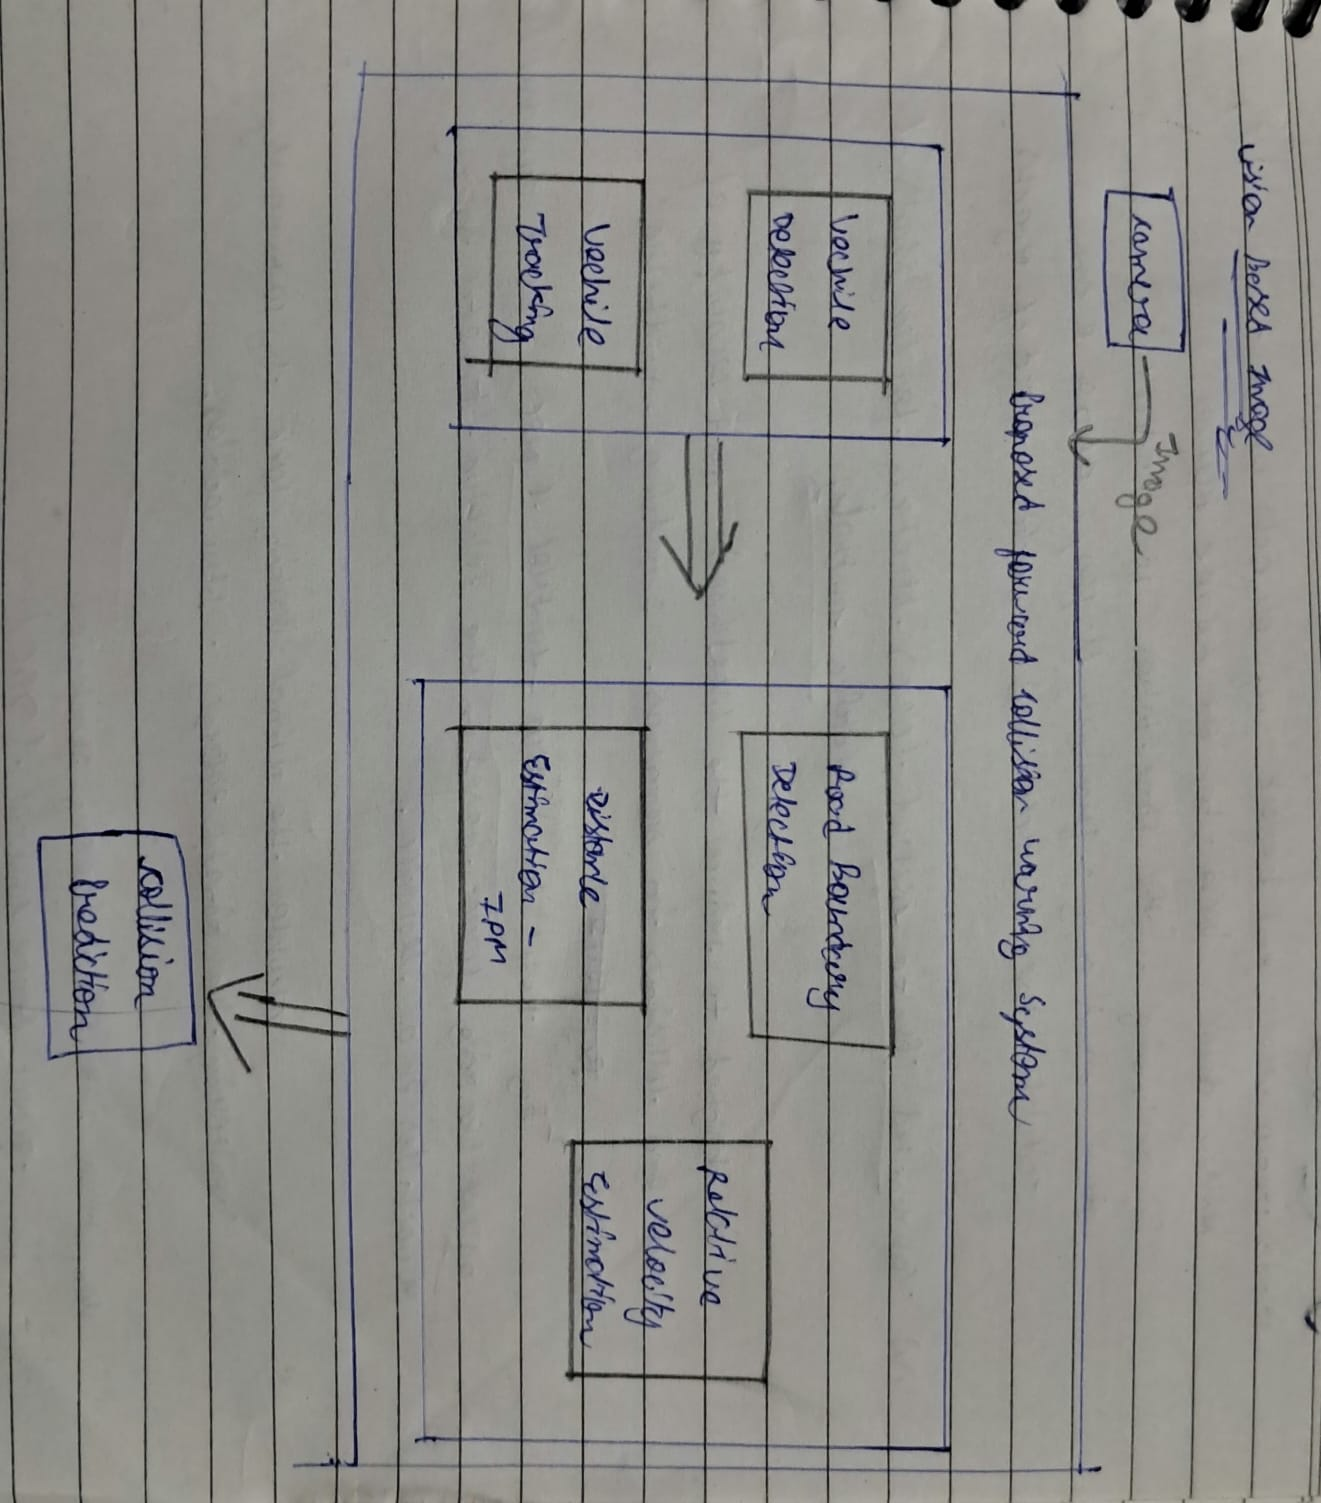
\includegraphics[scale=0.3]{VISION.jpg}
\caption{VISION BASED}
\label{fig_VISION_Based}
\end{figure}

\subsection{LIDAR-Based Systems}

This experiment demonstrates the integration of a LiDAR sensor and DC motors on a Micro-Aerial Vehicle (MAV) for obstacle avoidance using an Arduino UNO. The system employs the TF-Luna LiDAR sensor, which operates on the Time of Flight (TOF) principle to measure the distance and relative velocity of obstacles. The sensor data is processed by the Arduino, which then controls the MAV's motors through an L293D motor driver IC. By adjusting motor speed and direction based on real-time obstacle detection, the system aids the MAV in avoiding collisions, a crucial aspect of Collision Avoidance Systems (CAS) (see Figure \ref{fig_LISP} for a visual representation of the setup).

The software calculates both distance and relative velocity of obstacles using serial communication with the LiDAR sensor. The Arduino implements a collision avoidance algorithm that adjusts motor thrust based on distance thresholds—reducing speed when obstacles are closer. This approach allows the MAV to respond effectively to nearby objects, enhancing its ability to navigate confined or dynamic environments. The integration of these components ensures the MAV can perform responsive, real-time obstacle avoidance.
\begin{figure}[h]
\centering
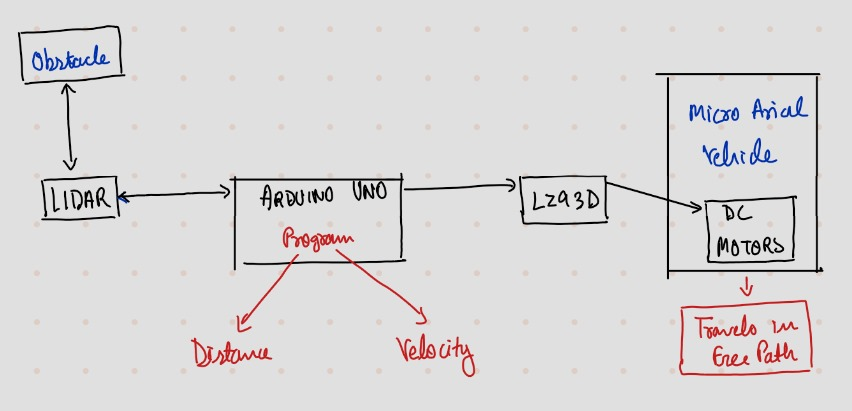
\includegraphics[scale=0.4]{LIDAR.jpg}
\caption{LIDAR}
\label{fig_LISP}
\end{figure}

\subsection{RADAR-Based Systems}
This dissertation focuses on the implementation of a RADAR-based collision avoidance system for unmanned aircraft systems (UAS) that are capable of increasing operational autonomy in outdoor environments. UAS rely strictly on pre-programmed commands and human supervision, as they do not possess high levels of safety for proper navigation in complex airspace. The proposed system utilizes radio detection and ranging technology, enabling UAS to detect potential collision threats, such as other UAVs, non-cooperatively without relying on a cooperative system like transponders. Its non-cooperative approach addresses the challenge of mid-air collisions, particularly in environments where traditional sensors cannot easily reach (refer to Figure \ref{fig_RADAR} for a visual representation of the proposed system).

This work includes several important contributions, namely: designing lightweight and energy-efficient hardware for the RADAR, suitable for a miniature UAS; nearly real-time detection and identification of nearby aircraft through their micro-Doppler signatures; and a computationally efficient collision avoidance algorithm based on identified threat information. Given the challenges related to size, power consumption, and cost of RADAR systems, this work aims to develop a more scalable and practically applicable solution to enhance the safety and autonomy of UASs in increasingly congested skies

\begin{figure}[h]
\centering
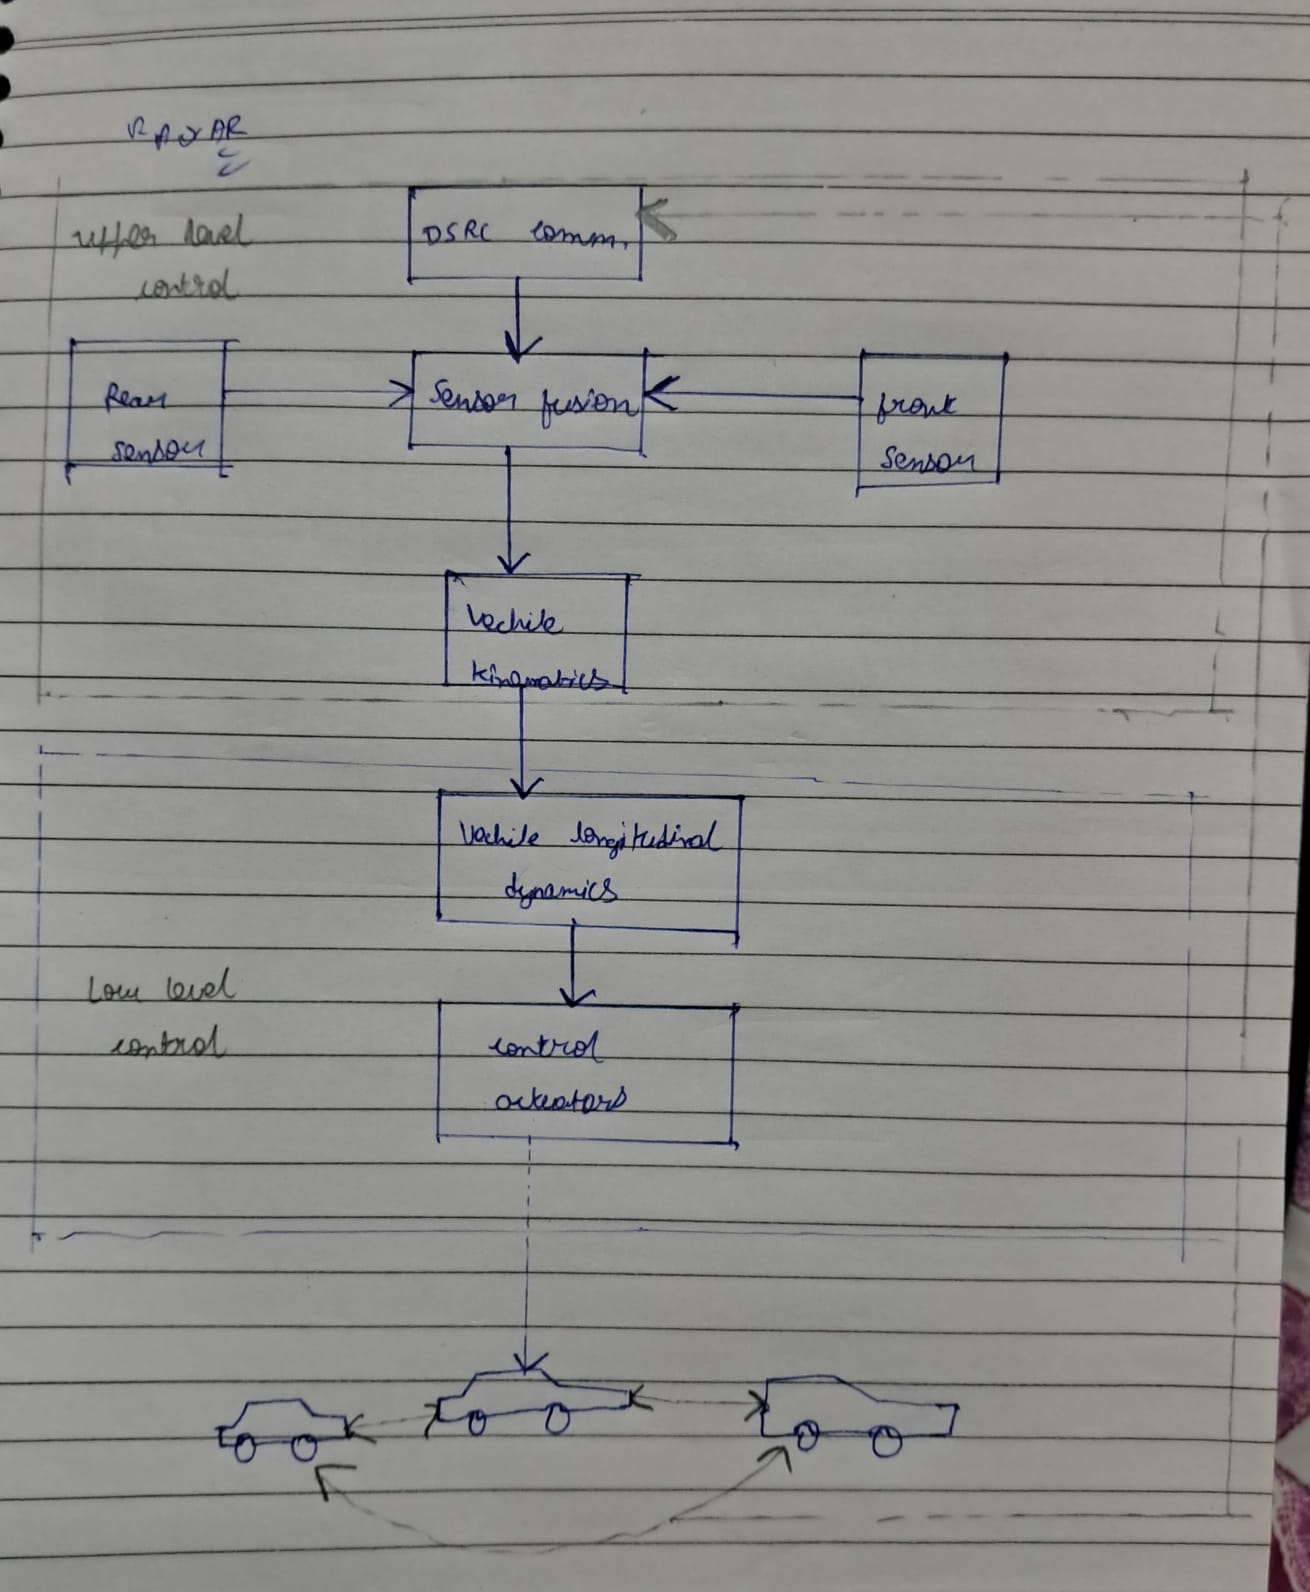
\includegraphics[scale=0.4]{RADAR.jpg}
\caption{RADAR}
\label{fig_RADAR}
\end{figure}
\subsection{Braking Control (Longitudinal)}

The article proposes a Coordinated Brake Control (CBC) strategy for mitigating rear-end collisions involving multiple vehicles using Model Predictive Control (MPC). By calculating the optimal braking force based on the relative kinetic energy between consecutive vehicles, the system aims to minimize the total impact energy in potential collisions. CBC outperforms other braking strategies, such as Direct Brake Control (DBC) and Linear Quadratic Regulator (LQR), in simulations, reducing both the risk and severity of collisions in multi-vehicle scenarios.

\subsection{Steering Control (Lateral)}

This paper presents an emergency steering control strategy for autonomous vehicles that addresses both collision avoidance and vehicle stabilization in critical situations. The proposed system uses a hierarchical control architecture with two layers: a decision-making layer that assesses collision risks and plans a safe path, and a motion control layer that ensures the vehicle follows this path while accounting for tire nonlinearity and external disturbances. The control is implemented using a backstepping sliding-mode controller, which estimates lateral tire forces to maintain stability during evasive maneuvers. Simulations and experiments show that this approach effectively avoids collisions while keeping the vehicle stable under dynamic conditions.

\subsection{Fuzzy Logic Control}
This paper explores the use of fuzzy logic for mobile robot obstacle avoidance in unknown and cluttered environments. The focus is on reactive navigation, which involves creating a mapping between sensor data and movement commands. The author highlights fuzzy logic as a viable alternative to traditional methods like potential fields or neural networks for building this mapping (see Figure \ref{fig_FUZZY} for a visual representation of the proposed approach). Using a behavior decomposition approach, the paper discusses how to establish fuzzy rules to control the robot. However, challenges such as oscillations and local minima remain. The author concludes that learning is essential for a robust navigation system, but fuzzy logic can help inject initial knowledge, reducing the need to start from scratch.
\begin{figure}[h]
\centering
\includegraphics[scale=0.26]{FUZZY.jpg}
\caption{FUZZY}
\label{fig_FUZZY}
\end{figure}

\subsection{Genetic Algorithm Optimization}

This paper presents a method for cooperative collision avoidance among multiple unmanned surface vehicles (USVs) using an improved genetic algorithm (GA). It addresses challenges in dynamic environments featuring obstacles by establishing models for USV motion and sensors, categorizing encounter scenarios, and formulating specific collision avoidance strategies. The GA is enhanced through retention, deletion, and replacement strategies to prevent local optima and speed up convergence. Additionally, the method optimizes the adjustment of velocity and heading, calculating the best path in real time.

Simulations demonstrate the effectiveness of the algorithm, confirming its ability to handle dynamic scenarios with and without communication among USVs. The improved GA offers advantages such as fast convergence, high stability, and low time complexity, making it suitable for other intelligent platforms. This work advances multi-objective optimization in USV navigation, overcoming key issues in traditional collision avoidance methods.

\subsection{Vehicle-to-Vehicle (V2V) Communication}

Vehicle to Vehicle (V2V) communication for collision avoidance in multi-copters is a critical system that enables drones to automatically communicate with each other to prevent crashes while flying in dense urban environments. This research by NASA specifically focuses on implementing V2V communication for drones operating in UTM (UAS Traffic Management) TCL4 - which represents the most complex level of drone traffic management in urban areas.
At its core, the system enables drones to exchange information with each other and coordinate their movements autonomously, similar to how modern cars can communicate to avoid accidents. This capability is especially important for drones flying Beyond Visual Line of Sight (BVLOS), where remote operators cannot directly see the aircraft. The research aims to develop reliable protocols and test them in high-fidelity simulations to ensure safe operation when multiple drones share the same airspace in cities.

\subsection{Vehicle-to-Infrastructure (V2I) Communication}

This paper reviews the role of Dedicated Short Range Communication (DSRC) technology within Intelligent Transportation Systems (ITS), focusing on Vehicle-to-Vehicle (V2V) and Vehicle-to-Infrastructure (V2I) communications. These systems, which fall under the broader category of Vehicle Ad-hoc Networks (VANET), aim to create safer urban environments for both drivers and pedestrians. While V2V and V2I technologies are still under development and not fully deployed worldwide, DSRC is a key communication method being explored. The paper describes the architecture of DSRC, including important standards like SAE J2735 and Basic Safety Messages (BSM). It also discusses various applications of DSRC, such as Emergency Electronic Brake Lights and Forward Collision Warnings.
The paper highlights that DSRC technology has advanced significantly from its initial use in electronic toll collection to a range of applications that enhance road safety. It operates at different frequency ranges, which are regulated by country-specific guidelines, impacting the coverage area of the communication. For example, in Europe, DSRC operates within the frequency range of 5.875 to 5.905 GHz, while in the U.S., it operates between 5.850 and 5.925 GHz. Understanding these technologies is essential for developing effective communication systems that can facilitate safer driving in increasingly crowded urban areas.

\subsection{Multi-Sensor Fusion}

This paper discusses the importance of accurately detecting and tracking objects, particularly for Remotely Piloted Aircraft Systems (RPAS), which are not yet fully equipped to operate safely in all airspaces due to the absence of certified Detect-and-Avoid (DAA) systems. DAA systems are essential for RPAS to safely navigate and avoid collisions with other aircraft or obstacles. The paper emphasizes the need for both cooperative (e.g., systems that share information like Automatic Dependent Surveillance-Broadcast or ADS-B) and non-cooperative detection methods (e.g., visual and thermal cameras, LIDAR, and acoustic sensors) to enhance the capabilities of these aircraft. Effective detection relies on high-performance sensors and robust communication, navigation, and surveillance (CNS) systems.
To improve object tracking, the paper proposes a Multi-Sensor Data Fusion (MSDF) approach that combines data from various sensors to create a more accurate understanding of an object's position and movement. Two advanced filtering techniques, the Unscented Kalman Filter (UKF) and the Particle Filter (PF), are used to estimate the state of objects, whether they are moving or stationary. Additionally, an artificial neural network is integrated into the system to help combine the information from the UKF and PF, utilizing statistical learning methods for better predictions. The paper also includes discussions on how visual and thermal image data can be effectively fused to improve detection capabilities further.

\subsection{Deep Learning Algorithms}

This paper presents a method for enhancing obstacle detection in robotic harvesters using deep learning, specifically by implementing a slimmed-down version of a convolutional neural network known as the Image Cascade Network (ICNet). The aim is to create a compact model suitable for real-time operation on devices with limited computational power, such as rice combine harvesters (refer to Figure \ref{fig_ICNet} for a visual representation of the proposed method). The authors applied a technique called Network Slimming, which reduces the size of the neural network by removing less important channels in its convolutional layers, resulting in a model that is 80% smaller yet maintains high accuracy. This pruned model was tested in real-world scenarios, demonstrating a high success rate of 96.6% in avoiding obstacles while processing images at a rate of 32.2 frames per second.

The introduction of semantic segmentation allows for pixel-by-pixel identification of various objects in the paddy fields, which is crucial for the harvester's navigation. Traditional image recognition methods fall short due to their reliance on manually crafted features and inability to adapt to varying environmental conditions. In contrast, the proposed method leverages the power of deep learning to achieve effective segmentation with reduced computational requirements. The results indicate that the approach not only enhances the harvester's obstacle detection capabilities but also contributes to safer and more efficient agricultural practices

\begin{figure}[h]
\centering
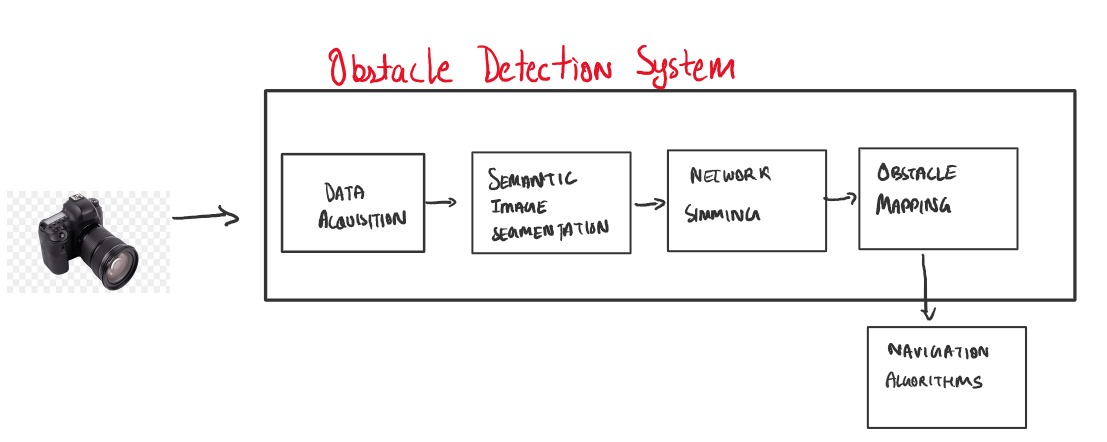
\includegraphics[scale=0.23]{Deep_learning_algorithim.jpg}
\caption{Deep Learning Algorithim}
\label{fig_ICNet}
\end{figure}
\subsection{Model Predictive Control (MPC)}

This paper discusses a Nonlinear Model Predictive Control (NMPC) system designed for autonomous vehicles to track their trajectories while avoiding obstacles on the road. The study compares two methods for obstacle avoidance and evaluates the NMPC performance in realistic driving scenarios that involve static obstacles on constrained roadways. To simplify the vehicle dynamics, the researchers used a bicycle model, which helps predict the future states of the vehicle during control. However, to accurately assess the vehicle's performance and test the NMPC, they utilized a more complex, high-fidelity nonlinear model known as CarSim in their simulations.
The results indicate that the NMPC controller effectively tracks the vehicle's path at typical road speeds while adhering to real-time processing requirements. One key finding is that longer prediction horizons—meaning the controller looks further into the future when making decisions—improve the vehicle's ability to respond to obstacles. With a longer look-ahead time, the NMPC can better plan maneuvers that minimize deviations from the desired path while avoiding obstacles, leading to safer and more efficient driving behaviour.

\subsection{Control Theory Approach}
The purpose is to create a controller (C) for a system (P) to behave in a manner acceptable according to (Spec), and rule out failure which may include crashing. Such an approach deals with the concepts of controllable events (managed by the controller) and uncontrollable events (emanating from the environment). The problem is how a winning strategy that keeps the system safe with respect to such uncontrollable events, which may be viewed as a controllable versus uncontrollable game.
Set Decision Diagrams (SDD) are in particular employed because of their capability to represent hierarchies and enhance the sharing of identical subcomponents. The aim is thus to use this framework to determine the controllability of Intelligent Transportation Systems (ITS), This complexity results in a combinatorial explosion of the possible configurations of the system. To solve this problem, the authors offer a promising encoding method which can efficiently encode realistic configurations and facilitate the management of scenarios with up to 150 vehicles in a four-lane section of a kilometer road. The experimental findings substantiate the validity of this approach.

\subsection{CARVNET}
The study underscores the significance of intelligent transportation systems (ITS) and vehicular ad hoc networks (VANETs) in enhancing road safety. The proposed system, named
intellegent collision avoidance routing (CARVNET), aims to prevent accidents by promptly notifying drivers and nearby emergency services when unusual driver behavior is detected. Simulation tests indicate that this system outperforms current methods, greatly enhancing communication efficiency and reducing delays. The research highlights the necessity of a strong accident avoidance mechanism to tackle the increasing number of road accidents and protect lives

\subsection{Vehicle Detection Technique}

It is necessary to use vehicle detection techniques in order to enhance road safety. Such systems use cameras and vision-based algorithms to detect vehicles, though the boundaries can be problematic due to factors like motos’ diverse physical configurations, multiple obstacles in the vicinity, and the presence of shadows or brightness changes.
At this point, we deal with such crucial issues as sensor choice, methods of determination and ways of further monitoring the target. It also deals with motorcycle detection methods and compares the effectiveness, price, and scope of various sensors.
With about 1.24 million overall road deaths recorded annually with many owing to driver distraction and exhaustion, the need for more advanced CASs is clear. The dialogue include several variables responsible for road accidents such as attention and child-like behavior from drivers, calling for more effective and cheap cost containment measures in the design of CAS systems. This is very important in reducing the risks of vulnerable road users such as motorcyclists.
VANET (Vehicular Ad Hoc Networks), as an important part of ITS (Intelligent Transportation System), enhances the road safety through the use of both Vehicle to Vehicle (V2V) and Vehicle to Infrastructure (V2I) communications. To implement a communications architecture where vehicles communicate with roadside units (RSUs) to facilitate long-distance data transfer, Wi-Fi and cellular networks are integrated within these systems.
\subsection{Speed-based lane changing collision avoidance}
The paper introduces a straightforward stereo vision system designed for speed-based lane detection and classification, aimed at enhancing Forward Collision Warning (FCW) in Advanced Driver Assistance Systems (ADAS). It employs a unique lane model developed in Hough Space, which effectively addresses challenges such as uneven road surfaces and varying lane configurations. By analyzing stereo images, the system can identify and classify lanes (such as dashed or solid) using a Convolutional Neural Network (CNN) that has been trained on a specific dataset. This capability enables the ego-car to determine its position and assess potential collision distances.

Moreover, the stereo vision technology allows the system to collect 3D data, generating obstacle masks that minimize distractions from roadside objects. This results in more precise lane detection, ensuring the vehicle is aware of safe driving areas. The system operates in real-time at a frequency of 15 Hz and demonstrates a high success rate in detecting and classifying lanes across various driving conditions. By utilizing stereo cameras instead of costly sensors like Lidar, this method remains budget-friendly while maintaining reliability, particularly in structured environments.
\subsection{ToA-based algorithm}

It aims to tackle transportation inefficiencies by focusing on speed-based lane changing, collision avoidance, and Time of Arrival (ToA) localization within Vehicular Ad-hoc Networks (VANETs). To address the limitations of traditional GPS systems, particularly in areas with weak signals, a ToA-based algorithm is developed for reliable vehicle positioning.

The system incorporates automatic braking and camera-based surveillance to enhance collision avoidance. Given the significant economic and environmental costs associated with traffic congestion, this ITS seeks to improve traffic flow through Vehicle-to-Vehicle (V2V) and Vehicle-to-Infrastructure (V2I) communication. The architecture consists of interconnected vehicles that exchange critical data, which is relayed to Road Side Units (RSUs) and subsequently sent to a cloud-based central server. This setup enables smart traffic management and monitoring, ultimately promoting safer and more efficient transportation systems.

\subsection{Sustainable Transpotation in IoV}
The sustainable transportation framework in the Internet of Vehicles (IoV) reduces pollution and enhances safety by connecting vehicles, infrastructure, and users. It integrates electric vehicles, smart grid technology, and intelligent traffic systems to address environmental challenges.

Key components include renewable energy-powered electric transport, efficient smart grids, and optimized EV designs with advanced charging stations. Intelligent traffic systems manage congestion, while public transport and car-sharing options offer sustainable alternatives. The K-bus project, using ultracapacitor batteries for fast charging, further minimizes environmental impact, creating eco-friendly transportation that prioritizes safety
\subsection{NLP methods in IoV}

The paper "Intelligent Transportation Systems (ITS): A Systematic Review Using a Natural Language Processing (NLP) Approach" presents a framework for conducting systematic reviews of ITS research, incorporating essential NLP techniques that improve literature analysis.

Named Entity Recognition (NER) is used to pinpoint and classify relevant terms from a large collection of research articles. The authors created a custom NER model utilizing the IOB (Inside-Outside-Beginning) tagging format, employing the SpaCy library and training it on a tailored dataset of ITS-related terms. This approach enables precise labeling of documents as either relevant or irrelevant based on the identified entities.

Latent Dirichlet Allocation (LDA) functions as a generative statistical model for topic modeling, organizing documents into topics by examining word co-occurrence. The authors refined LDA by adjusting hyperparameters such as the number of topics and coherence scores, which facilitates the grouping of similar articles based on common themes. Furthermore, Continuous Skip-Gram word embedding captures the context of words by converting them into vector representations, highlighting relationships among terms within each topic cluster. This reduces the need for manual reading, making it particularly effective for efficiently analyzing large datasets

\subsection{ Machine Learning in IoV}

The proposed framework for machine learning (ML)-enhanced Intelligent Transportation Systems (ITS) aims to address the growing needs of smart cities by optimizing traffic management, safety, energy efficiency, and pollution control. This approach includes an ML-driven model for ITS applications, emphasizing autonomous vehicles, traffic flow optimization, and network security.
To support ITS scalability and improve quality of service, the framework utilizes supervised and unsupervised ML algorithms to analyze and manage large datasets. Cooperative driving models, hazard warning systems, and predictive maintenance are integrated to enhance safety and streamline traffic. Furthermore, advanced neural networks are employed to refine route optimization and mitigate congestion in real-time. The model’s architecture provides robust solutions for dynamic traffic environments, overcoming traditional data processing limitations. Ultimately, the ML-based ITS framework contributes to smarter, safer transportation networks that are both adaptive and efficient.

\section{Discussion: Current Challenges and Suggested Improvements}
\begin{enumerate}
\item Limitations of Sensors:
Problem:
Vision systems do not perform well in low light or bad weather.
LIDAR and RADAR is expensive and prone to be affected by its environment.
Single sensors fail or output wrong data.
Improvement:
Use multiple sensors, such as LIDAR, RADAR, and cameras, to generate better results.
Advanced deep learning might enable improving sensors, as it reduces noise and improves quality of data.

\item Computational Complexity:
Problem:
The problems facing the V2V and V2I systems are high delay and security hazards.
These issues make it hard to expand these systems widely.
Improvement:
Improve communication through 5G networks with faster and safer connections.
Implement blockchain technology on V2X systems in order to secure data, thus minimizing hacking risks.

\item Flexibility towards Dynamic Environments:
Problem:
Current methods such as Fuzzy Logic and Genetic Algorithms are not adaptive to changing situations rapidly.
Enhancement:
Reinforcement learning (RL) can adapt and enable systems to learn from real driving experiences to change their actions.
Combining RL with traditional methods such as MPC can improve decision-making in complex situations.
\item Cost Constraints:
Problem:
The high prices of LIDAR, RADAR, and advanced computers limit the use of collision avoidance systems, especially in cheaper cars.
Improvement:
New solid-state LIDAR and low-cost RADAR will further help reduce costs.
Cloud-based processing, resource sharing, and similar capabilities also reduce the cost for real-time decision-making.
\end{enumerate}
\section{Table}

The following table summarizes various techniques and their key components, strengths, and limitations in collision avoidance systems. The table is long, so it has been resized for better readability.
\onecolumn
\begin{longtable}{|p{3cm}|p{4cm}|p{3cm}|p{3cm}|p{3cm}|} % Added p{3cm} for the new column
\hline
\textbf{Technique} & \textbf{Key Components} & \textbf{Strengths} & \textbf{Limitations} & \textbf{References} \\ \hline
\endfirsthead % Header for the first page
\hline
\textbf{Technique} & \textbf{Key Components} & \textbf{Strengths} & \textbf{Limitations} & \textbf{References} \\ \hline
\endhead % Header for subsequent pages
\hline
\endfoot % Footer for all pages
\hline
\endlastfoot % Last footer

Vision-Based Systems & Cameras, Image Processing, Neural Networks & Cost-effective, good for lane and pedestrian detection & Limited in low-light or adverse weather conditions & \citet{park2023} \\ \hline
LIDAR-Based Systems & Light Detection and Ranging Sensors, Point Cloud Processing & High accuracy in various weather conditions & Expensive, sensitive to environmental interference & \citet{kollabathula2023}  \\ \hline
RADAR-Based Systems & Radio Waves, Doppler Effect for Speed Estimation & Effective in poor visibility and long-range detection & Lower resolution compared to LIDAR & \citet{moses2013} \\ \hline
Braking Control (Longitudinal) & Speed Sensors, Adaptive Cruise Control (ACC), Emergency Braking Systems & Reduces speed effectively to avoid collisions & Requires large safety distances, ineffective in short stopping distances & \citet{wang2015} \\ \hline
Steering Control (Lateral) & Steering Actuators, Model Predictive Control (MPC), Path Planning Algorithms & Good for avoiding obstacles in emergencies & May cause lateral instability in high-speed conditions & \citet{he2019} \\ \hline
Fuzzy Logic Control & Fuzzy Controllers, Rule-Based Systems, Driver Behavior Modeling & Adapts to uncertain environments, mimics human decisions & Rule optimization is complex, dependent on accurate rule sets & \citet{reignier1994} \\ \hline
Genetic Algorithm Optimization & Genetic Algorithms, Binary Coding of Control Rules, Fitness Functions & Dynamically optimizes control rules & Computationally expensive, convergence issues with large datasets & \citet{wang2021} \\ \hline
Vehicle-to-Vehicle (V2V) Communication & Wireless Communication (DSRC, 5G), Cooperative Adaptive Cruise Control (CACC) & Enables cooperative driving, reduces intersection accidents & Limited by communication delays, needs wide-scale deployment & \citet{chakrabarty2019} \\ \hline
Vehicle-to-Infrastructure (V2I) Communication & Communication with traffic signals and road infrastructure & Improves traffic flow, proactive hazard identification & Expensive infrastructure upgrades, data security concerns & \citet{khan2022} \\ \hline
Multi-Sensor Fusion & Integration of data from LIDAR, RADAR, Cameras, Ultrasonic Sensors & Enhanced decision-making through multiple data sources & Complex data processing, sensor discrepancies may lead to inaccuracies & \citet{cappello2015} \\ \hline
Deep Learning Algorithms & Convolutional Neural Networks (CNN), Reinforcement Learning (RL), Object Detection & Learns from real-world scenarios, high adaptability & Requires large datasets, risk of overfitting & \citet{li2020} \\ \hline
Model Predictive Control (MPC) & Real-Time Optimization of Vehicle Paths, Dynamic Models of Vehicle and Environment & Precise trajectory planning, adaptable in real-time & High computational demand, unsuitable for highly dynamic environments & \citet{abbas2017} \\ \hline
Discrete Control Theory & Discrete-Time Controllers, State Feedback, Linear Control Design & Well-defined for dynamic systems & Limited applicability in nonlinear systems & \citet{berard2008} \\ \hline
Intelligent Collision Avoidance Routing (CARVNET) & Routing Protocols for VANETs, Adaptive Network Algorithms & Avoids high-traffic or accident-prone areas & Challenging to scale, requires robust infrastructure & \citet{kaur2022} \\ \hline
Vehicle Detection and Tracking & Sensor Fusion, Detection Algorithms, Tracking Filters (e.g., Kalman) & Accurate vehicle detection in dynamic environments & Computationally expensive, depends on sensor accuracy & \citet{mukhtar2015}\\ \hline
Speed-Based Lane Changing and Collision Avoidance & Speed Sensors, Lane Detection, Dynamic Lane Assignment Algorithms & Improves lane-changing decisions based on speed & High computational demand, needs real-time vehicle data & \citet{song2018} \\ \hline
Time of Arrival (ToA) Based Localization for VANETs & ToA Sensors, Signal Processing Algorithms, VANET Communication & Real-time vehicle positioning for collision prevention & Sensitive to signal noise, requires reliable networks & \citet{naikcloud2019} \\ \hline
Sustainable Transportation in IoV & Green Routing Algorithms, Energy-Efficient Driving, Eco-Driving Support Systems & Optimizes fuel consumption, reduces environmental impact & Complex route planning, needs advanced infrastructure & \citet{balasubramaniam2017} \\ \hline
Natural Language Processing (NLP) Methods in IoV & NLP Algorithms, Communication Systems for Command Interpretation & Enables voice-based control, optimizes user interaction & Potential misinterpretation in critical moments & \citet{putri2021} \\ \hline
Machine Learning in IoV & Supervised, Unsupervised Learning, Real-Time Data Processing & Learns to optimize collision avoidance from data & Prone to overfitting without careful tuning &\citet{yuan2022} \\ \hline

\end{longtable}
\twocolumn
\section{conclusion}
While there have been notable advancements in collision avoidance techniques for Intelligent Transportation Systems (ITS), several challenges still persist. Current systems encounter problems related to sensor reliability, high computational demands, communication infrastructure, and their ability to adapt to changing environments. To enhance these systems, future research should prioritize the integration of multi-sensor data, the use of edge computing and machine learning methods, and the improvement of communication networks. By tackling these issues, we can create safer and more efficient transportation systems. This comprehensive analysis should provide a strong basis for your report on collision avoidance techniques in Intelligent Transportation Systems. You can elaborate on each section by exploring specific case studies, simulation outcomes, or ongoing initiatives.
\bibliographystyle{plainnat}
\bibliography{references} 
%\printbibliography[heading=bibintoc]
\end{document}
